\documentclass{article}
\usepackage{amsmath}
\usepackage{tikz}
\usetikzlibrary{matrix}

\begin{document}

\begin{center}
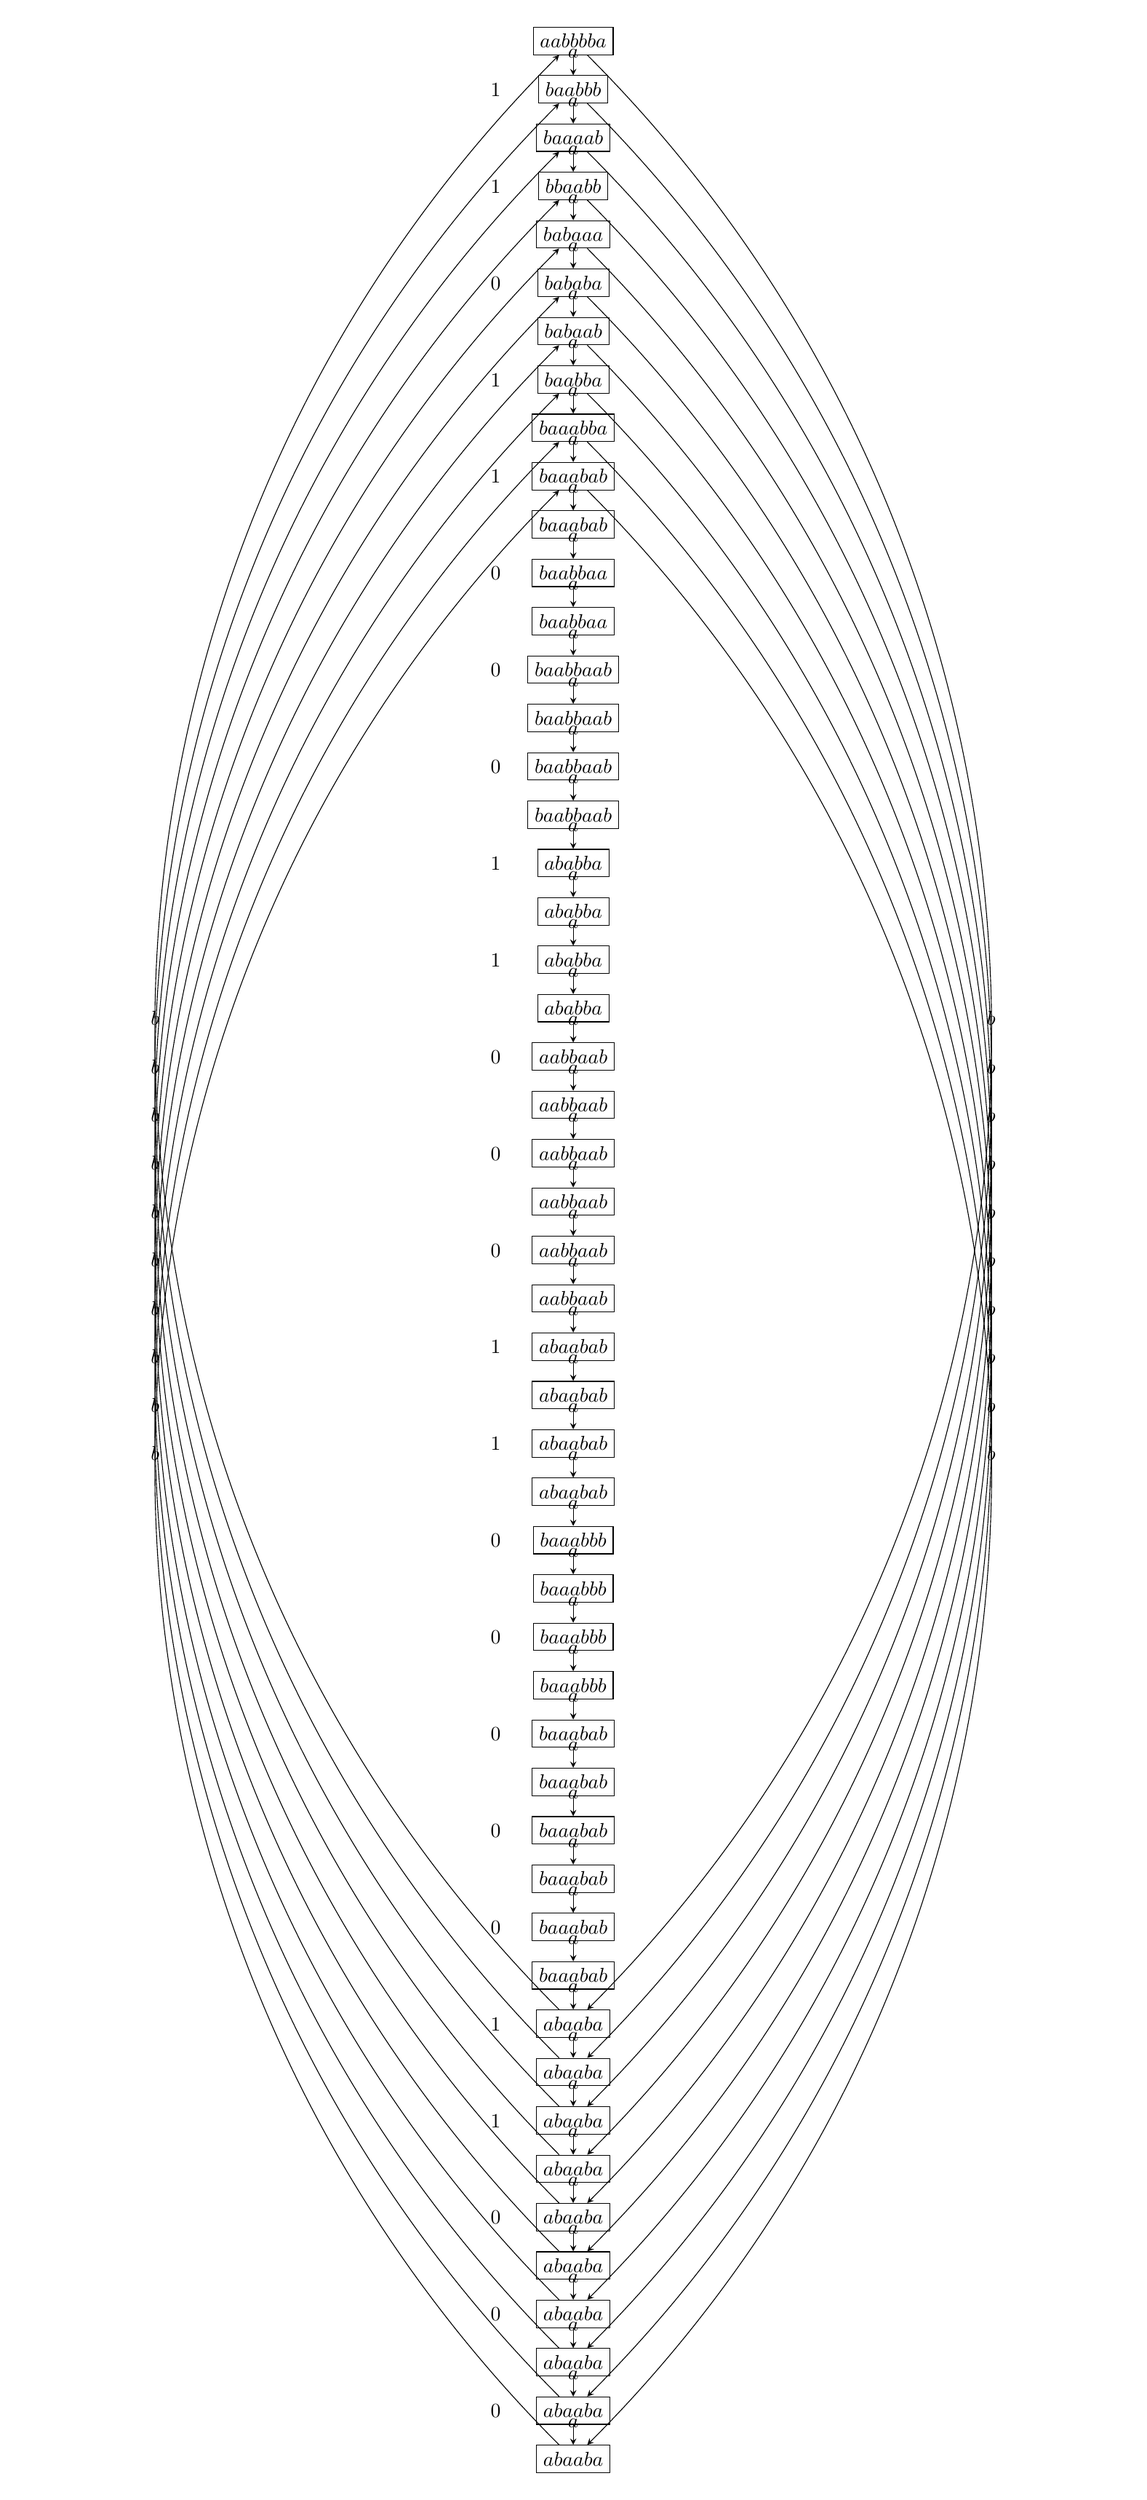
\begin{tikzpicture}[node distance=1cm]
    \matrix (m) [matrix of nodes, row sep=1em, column sep=1em] {
        & \node[draw] (a1) {$aabbbba$}; & \\
        1 & \node[draw] (a2) {$baabbb$}; & \\
        & \node[draw] (a3) {$baaaab$}; & \\
        1 & \node[draw] (a4) {$bbaabb$}; & \\
        & \node[draw] (a5) {$babaaa$}; & \\
        0 & \node[draw] (a6) {$bababa$}; & \\
        & \node[draw] (a7) {$babaab$}; & \\
        1 & \node[draw] (a8) {$baabba$}; & \\
        & \node[draw] (a9) {$baaabba$}; & \\
        1 & \node[draw] (a10) {$baaabab$}; & \\
        & \node[draw] (a11) {$baaabab$}; & \\
        0 & \node[draw] (a12) {$baabbaa$}; & \\
        & \node[draw] (a13) {$baabbaa$}; & \\
        0 & \node[draw] (a14) {$baabbaab$}; & \\
        & \node[draw] (a15) {$baabbaab$}; & \\
        0 & \node[draw] (a16) {$baabbaab$}; & \\
        & \node[draw] (a17) {$baabbaab$}; & \\
        1 & \node[draw] (a18) {$ababba$}; & \\
        & \node[draw] (a19) {$ababba$}; & \\
        1 & \node[draw] (a20) {$ababba$}; & \\
        & \node[draw] (a21) {$ababba$}; & \\
        0 & \node[draw] (a22) {$aabbaab$}; & \\
        & \node[draw] (a23) {$aabbaab$}; & \\
        0 & \node[draw] (a24) {$aabbaab$}; & \\
        & \node[draw] (a25) {$aabbaab$}; & \\
        0 & \node[draw] (a26) {$aabbaab$}; & \\
        & \node[draw] (a27) {$aabbaab$}; & \\
        1 & \node[draw] (a28) {$abaabab$}; & \\
        & \node[draw] (a29) {$abaabab$}; & \\
        1 & \node[draw] (a30) {$abaabab$}; & \\
        & \node[draw] (a31) {$abaabab$}; & \\
        0 & \node[draw] (a32) {$baaabbb$}; & \\
        & \node[draw] (a33) {$baaabbb$}; & \\
        0 & \node[draw] (a34) {$baaabbb$}; & \\
        & \node[draw] (a35) {$baaabbb$}; & \\
        0 & \node[draw] (a36) {$baaabab$}; & \\
        & \node[draw] (a37) {$baaabab$}; & \\
        0 & \node[draw] (a38) {$baaabab$}; & \\
        & \node[draw] (a39) {$baaabab$}; & \\
        0 & \node[draw] (a40) {$baaabab$}; & \\
        & \node[draw] (a41) {$baaabab$}; & \\
        1 & \node[draw] (a42) {$abaaba$}; & \\
        & \node[draw] (a43) {$abaaba$}; & \\
        1 & \node[draw] (a44) {$abaaba$}; & \\
        & \node[draw] (a45) {$abaaba$}; & \\
        0 & \node[draw] (a46) {$abaaba$}; & \\
        & \node[draw] (a47) {$abaaba$}; & \\
        0 & \node[draw] (a48) {$abaaba$}; & \\
        & \node[draw] (a49) {$abaaba$}; & \\
        0 & \node[draw] (a50) {$abaaba$}; & \\
        & \node[draw] (a51) {$abaaba$}; & \\
    };
    \path[-stealth]
        (a1) edge node[above] {$a$} (a2)
        (a2) edge node[above] {$a$} (a3)
        (a3) edge node[above] {$a$} (a4)
        (a4) edge node[above] {$a$} (a5)
        (a5) edge node[above] {$a$} (a6)
        (a6) edge node[above] {$a$} (a7)
        (a7) edge node[above] {$a$} (a8)
        (a8) edge node[above] {$a$} (a9)
        (a9) edge node[above] {$a$} (a10)
        (a10) edge node[above] {$a$} (a11)
        (a11) edge node[above] {$a$} (a12)
        (a12) edge node[above] {$a$} (a13)
        (a13) edge node[above] {$a$} (a14)
        (a14) edge node[above] {$a$} (a15)
        (a15) edge node[above] {$a$} (a16)
        (a16) edge node[above] {$a$} (a17)
        (a17) edge node[above] {$a$} (a18)
        (a18) edge node[above] {$a$} (a19)
        (a19) edge node[above] {$a$} (a20)
        (a20) edge node[above] {$a$} (a21)
        (a21) edge node[above] {$a$} (a22)
        (a22) edge node[above] {$a$} (a23)
        (a23) edge node[above] {$a$} (a24)
        (a24) edge node[above] {$a$} (a25)
        (a25) edge node[above] {$a$} (a26)
        (a26) edge node[above] {$a$} (a27)
        (a27) edge node[above] {$a$} (a28)
        (a28) edge node[above] {$a$} (a29)
        (a29) edge node[above] {$a$} (a30)
        (a30) edge node[above] {$a$} (a31)
        (a31) edge node[above] {$a$} (a32)
        (a32) edge node[above] {$a$} (a33)
        (a33) edge node[above] {$a$} (a34)
        (a34) edge node[above] {$a$} (a35)
        (a35) edge node[above] {$a$} (a36)
        (a36) edge node[above] {$a$} (a37)
        (a37) edge node[above] {$a$} (a38)
        (a38) edge node[above] {$a$} (a39)
        (a39) edge node[above] {$a$} (a40)
        (a40) edge node[above] {$a$} (a41)
        (a41) edge node[above] {$a$} (a42)
        (a42) edge node[above] {$a$} (a43)
        (a43) edge node[above] {$a$} (a44)
        (a44) edge node[above] {$a$} (a45)
        (a45) edge node[above] {$a$} (a46)
        (a46) edge node[above] {$a$} (a47)
        (a47) edge node[above] {$a$} (a48)
        (a48) edge node[above] {$a$} (a49)
        (a49) edge node[above] {$a$} (a50)
        (a50) edge node[above] {$a$} (a51)
        (a1) edge[bend left=45] node[above] {$b$} (a42)
        (a42) edge[bend left=45] node[above] {$b$} (a1)
        (a2) edge[bend left=45] node[above] {$b$} (a43)
        (a43) edge[bend left=45] node[above] {$b$} (a2)
        (a3) edge[bend left=45] node[above] {$b$} (a44)
        (a44) edge[bend left=45] node[above] {$b$} (a3)
        (a4) edge[bend left=45] node[above] {$b$} (a45)
        (a45) edge[bend left=45] node[above] {$b$} (a4)
        (a5) edge[bend left=45] node[above] {$b$} (a46)
        (a46) edge[bend left=45] node[above] {$b$} (a5)
        (a6) edge[bend left=45] node[above] {$b$} (a47)
        (a47) edge[bend left=45] node[above] {$b$} (a6)
        (a7) edge[bend left=45] node[above] {$b$} (a48)
        (a48) edge[bend left=45] node[above] {$b$} (a7)
        (a8) edge[bend left=45] node[above] {$b$} (a49)
        (a49) edge[bend left=45] node[above] {$b$} (a8)
        (a9) edge[bend left=45] node[above] {$b$} (a50)
        (a50) edge[bend left=45] node[above] {$b$} (a9)
        (a10) edge[bend left=45] node[above] {$b$} (a51)
        (a51) edge[bend left=45] node[above] {$b$} (a10);
    \end{tikzpicture}
\end{center}

\caption{One of the two cobounding maps \( X \to \mathbb{Z}/2\mathbb{Z} \) on the Thue--Morse shift for the morphism \( \varphi: \{a,b\}^* \to \mathbb{Z}/2\mathbb{Z} \), \( \varphi(a)=1 \), \( \varphi(b)=0 \). The map is constant on cylinders of length 7.}
\label{fig:cobounding_map_thue_morse}
\end{document}